\section{Results}
\label{results}

\subsection{Comparison with optimal data}

The grid search over parameter values of the heuristic models yields results which are hard to interpret. Therefore, we choose the parameter value given in \cite{shunan2011} and plot the agreement of the heuristic models with the human and optimal data as follows.

\begin{figure}[h]
\begin{center}
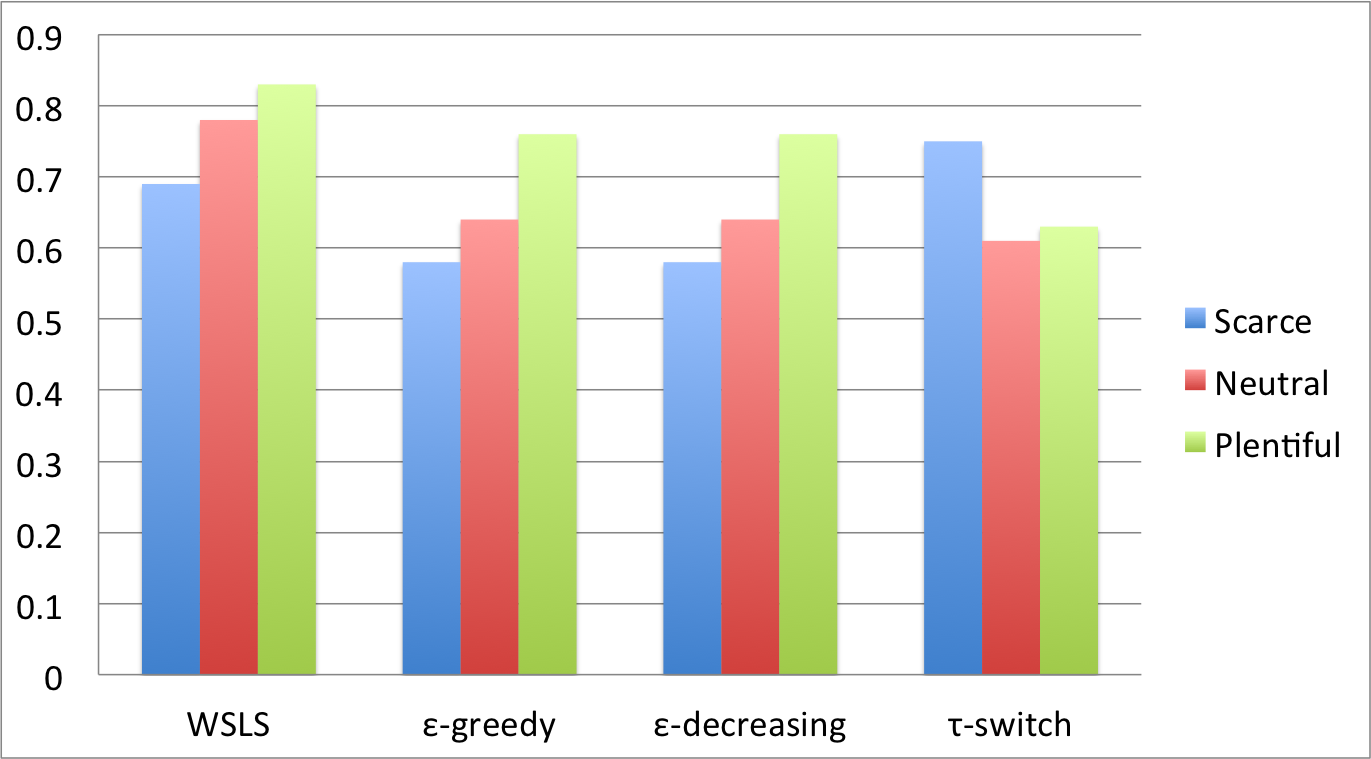
\includegraphics[scale=0.5]{optimalVsHeuristicNoTitle}
\caption{\small \sl \label{plot1} Agreement of Heuristic Models with Optimal Model}
\end{center}
\end{figure}

Figure~\ref{plot1} shows the agreement of each of the heuristic models with the decisions obtained using the optimal model, for each of the three environment settings. The agreement with optimal is maximum for the `plentiful' environment for most of the heuristics, which agrees with the results in \cite{shunan2011}.

\subsection{Comparison with human data}
\begin{figure}[H]
\begin{center}
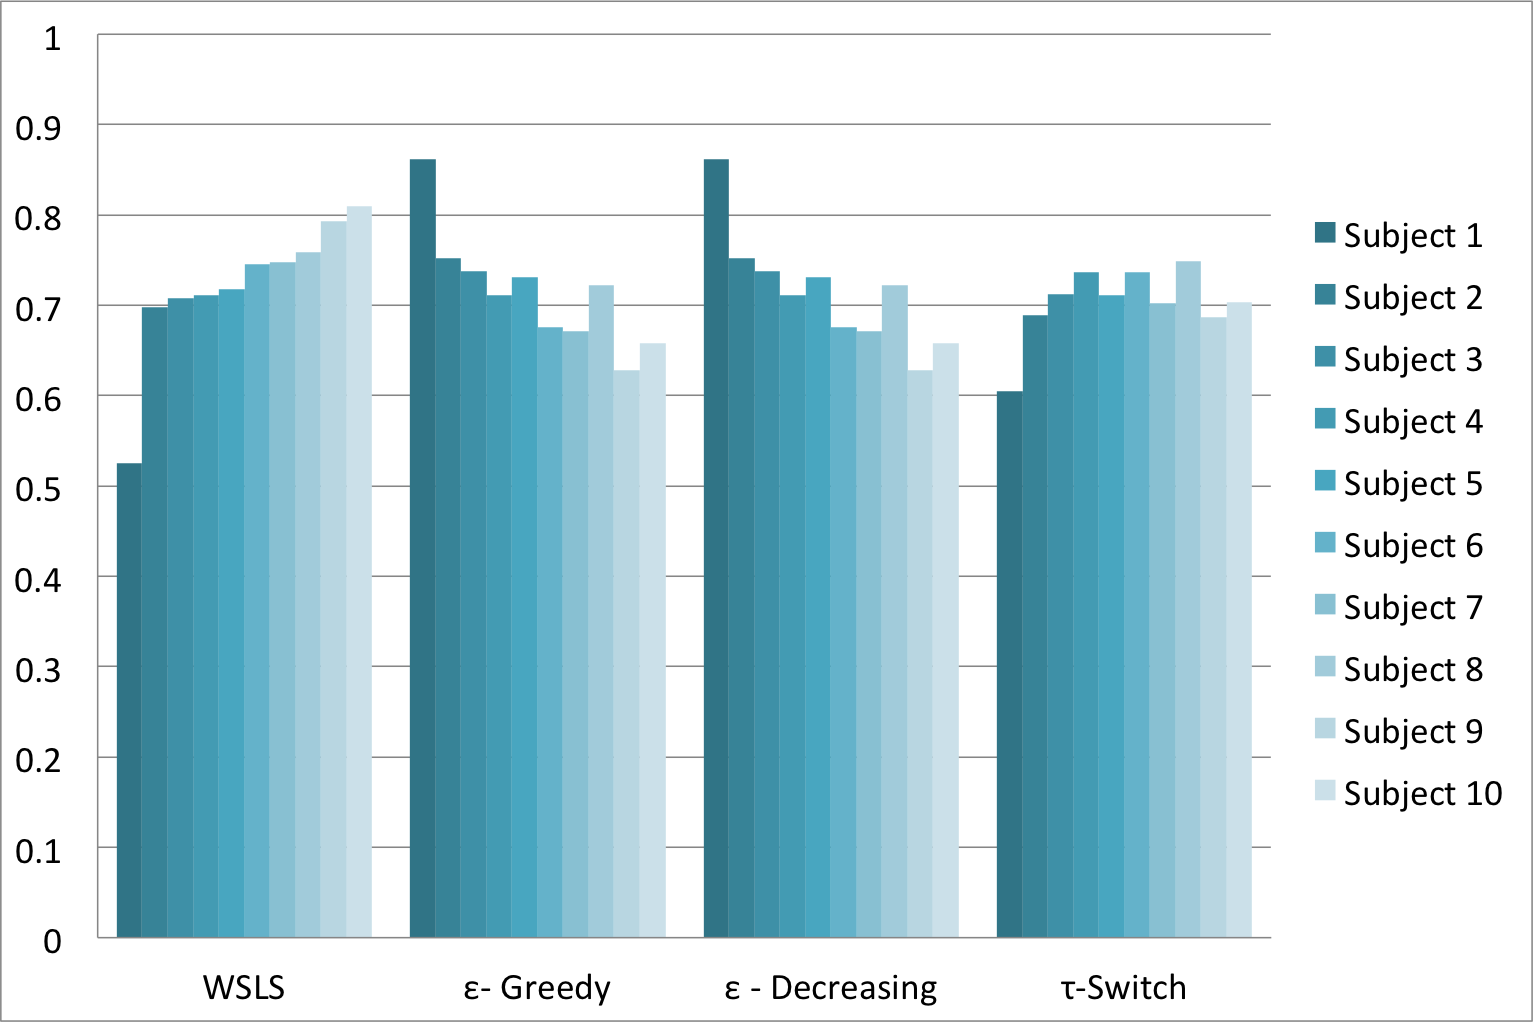
\includegraphics[scale=0.5]{humanVsHeuristicNoTitle}
\caption{\small \sl \label{plot2} Agreement of Heuristic Models with Human Data}
\end{center}
\end{figure}

Figure~\ref{plot2} shows the agreement of the heuristics with the human data for each of the 10 subjects. The 10 bars for the WSLS have been sorted in increasing order of agreement, while the bars for the remaining heuristics follow this sorted order of the participants.
